\section{{Case Study}\label{sec:introduction}}

\subsection{Stressor Events and Posting Behaviors}
\begin{figure}
\centering
\includegraphics[width=\linewidth,height=5cm]{figs/4time_line.eps}
\caption{Distribution of grade-oriented study-related stressful routine events at Taicang High School}
\label{fig:eventDistribution}
\end{figure}

\setlength{\tabcolsep}{2.5pt}
\begin{table}
\begin{footnotesize}
\begin{center}
\begin{tabular}{|c|c|c|c|} \hline
%&\multirow{2}{2cm}{\textbf{Number of Involved Students}}
%&\multirow{2}{2cm}{\textbf{Number of \colorbox{yellow}{posts}}}
%&\multirow{2}{2cm}{\textbf{Number of Stressor Events}}\\
& \textbf{Number of} & \textbf{Number of} & \textbf{Number of} \\
& \textbf{Involved Students} & \textbf{Posts} & \textbf{Stressor Events} \\ \hline
Grade 1 & 88 & 13311 & 38 \\\hline
Grade 2 & 124 & 10488 & 48\\\hline
Grade 3 & 107 &  5433 & 36 \\\hline
Total       &  -  & 29232 & 122 \\ \hline
\end{tabular}
\caption{Number of involved students, posts, and stressor events for three grades in the user study}
\label{tab:periodSummary}
\end{center}
\end{footnotesize}
\end{table}

\emph{Stressor Events.} To empirically study the correlation between stressor events and teens' abnormal posting behaviors,
we conduct a user study at Taicang High School, a key senior high school in Zhejiang Province of China.
The school publishes its weekly agenda regularly on the school's official web site one week in advance
to let students, teachers, and parents know school schedules beforehand.
We find 273 school events from January 1, 2012 to February 1, 2015,
where the majority are study-related. We further filter out 122 stressful study-related events such as
examination, contest, result notification, etc.
Table~\ref{tab:schoolEventSummary} lists some typical events, their duration, significance in evaluating students' school performance,
and total occurring frequencies during the observed three years.
Fig.~\ref{fig:eventDistribution} shows the distribution of
study-related stressor events, which happen to students when they are at different grades.
As these events are routine and grade-oriented, each year, students of the same grade experience the same events as those in previous years.
On average, 2-3 stressor events take place each month for each grade of students.

\emph{Posts.}
We identify 124 students who are active Tencent Weibo users
(registered before January 1st, 2012 and posted more than 100 posts on the microblog)
in Taicang Senior High School.
All students are anonymous, and all posts are public.
From January 1, 2012 to February 1, 2015, they posted 29,232 posts in total.
The average post number is 236 posts, 1,387 posts maximally, and 104 posts minimally.
Table~\ref{tab:periodSummary} shows for each grade, the number of involved students in the observed
three years, number of posts from the students, and number of stressor events.

Applying the stress detection function~\cite{HIS,LHJ} to each post $w_t$ posted at time $t$,
we can sense teen's stress level in the dimension of school, family, peer-relation, self-cognition, or romantic-relation, denoted as
$stress(t,w)$=$(t,C,l)$, where $C \subset {\cal C}$=$\{c^1,c^2,\cdots,c^6\}$,
corresponding to stress category {\emph{school}, \emph{family}, \emph{peer-relation},
\emph{self-cognition}, \emph{romantic-relation}, and \emph{unknown},
and $l \in {\cal L}=\{0,1,2,3,4,5\}$, corresponding to
\emph{none, very light, light, moderate, strong, very strong} stress level.
If no categorical words appear in the post, we assign the detected stress level
to an ``\emph{unknown}" category.
We call $w$  a \textbf{stressful post}, if the detected stress $l>0$,
and otherwise, it is called a \textbf{non-stressful post}.

\emph{Relationship between Stressor Events and Stressful Posts.}
To examine the influence of stressor events upon students' posting behavior,
we partition the whole observation window into two complementary sets:
\emph{stressor-event period set} and \emph{non-stressor-event period set}. %$INE$.
Due to the continuity of human's emotion, we include a $\Delta_t$-day window on either side of
a stressor-event period. The computation of $\Delta_t$ is based on the significance of the event and
event duration. In this study, $\Delta_t$=$Sigificance$*$Duration$.
The basic time unit is day.
If overlap exists between two stressor-event periods,
we collapse them into one.

Then, for each student, we look at how different his/her posting behavior is during stressor-event periods and non-stressor-event periods through the following four
indicators:

\comment{
\begin{itemize}
\item number of tweets posted per day $R_{tweet}$:
\item number of stressful tweets posted per day $R_{stress\_tweet}$;
\item accumulated stress level reflected from posted tweets per day $R_{stress\_level}$;
\item proportion of stressful tweets over the whole tweets per day $R_{stress\_proportion}$=$R_{tweet}$/$R_{stress\_tweet}$.
\end{itemize}
}

\begin{itemize}
\item $R_{\#post}$: ratio of average number of posts per day during stressor-event periods and non-stressor-event periods;
\item $R_{\#stress\_post}$: ratio of average number of stressful posts per day during stressor-event periods and non-stressor-event periods;
\item $R_{\#stress\_level}$: ratio of average accumulated stress level per day during stressor-event periods and non-stressor-event periods;
\item $R_{\#stress\_proportion}$: ratio of average stressful posts proportion per day during stressor-event periods and non-stressor-event periods, i.e.,
$R_{\#stress\_proportion}$=$\frac{R_{\#post}}{R_{\#stress\_post}}$.
\end{itemize}

If an indicator value is close to 1.0, the difference under this indicator during stressor and non-stressor-event
periods is small.

\begin{figure}
\centering
\includegraphics[width=\linewidth,height=5.5cm]{figs/ratioPeriod.eps}
\caption{Histograms of $R_{\#post},R_{\#stress\_post},R_{\#stress\_level}$ and $R_{\#stress\_proportion}$
 during stressor-event and non-stressor-event periods}
\label{fig:ratioPeriod}
\end{figure}

\begin{figure}
\centering
\includegraphics[width=\linewidth,height=5.5cm]{figs/ratioGrade.eps}
\caption{Histograms of $R_{\#stress\_post}$ for different grades' students during stressor-event and non-stressor-event periods}
\label{fig:ratioGrade}
\end{figure}

\subsection{Empirical Findings}
We plot the average histograms of the four ratios
\small{$R_{\#post}$, $R_{\#stress\_post}$, $R_{\#stress\_level}$, and $R_{\#stress\_proportion}$} for all the 124 students in Fig.~\ref{fig:ratioPeriod},
and find that all the four indicator values are more to the right of the ratio value 1.0,
especially for indicator $R_{\#stress\_post}$ (whose black curve skews to the right of ratio value 1.0 the most).
It shows that the students tend to post more stressful posts per day during stressful-event periods than non-stressful-event periods.
This phenomenon particularly holds for the final-year Grade 3's students, whose
black curve skews to the right of ratio value 1.0 the most, as shown in Fig.~\ref{fig:ratioGrade}.
Close to graduation and national college entrance exam, apparently,
the study-related events pressurize them the most than Grade 1 and 2's students.

This empirical finding helps us shape our problem solution:
a teen's posting behavior is different during stressor-event periods and non-stressor-event periods, and
higher ratio values of $R_{\#post}$, $R_{\#stress\_post}$, $R_{\#stress\_level}$, and $R_{\#stress\_proportion}$
exist during stressor-event periods than non-stressor-event periods.
By mining the information statistically, we may identify teen's stressful periods, from which
stressor events can be extracted.
